\section{Sviluppatori}
\subsection{UC 4.1 - Visualizzazione elenco frasi}
\begin{itemize}
\item[•]\textbf{Attori}: Sviluppatore;
\item[•]\textbf{Descrizione}: Lo sviluppatore visualizza un elenco di frasi accompagnate dalla data di creazione e dall’autore ordinate cronologicamente;
\item[•]\textbf{Precondizione}:  L'amministratore ha approvato l’utenza dello sviluppatore e lo sviluppatore si è autenticato nel sistema.
\item[•]\textbf{Postcondizione}: 
\item[•]\textbf{Flusso degli eventi principale}: Lo sviluppatore ha selezionato la voce relativa alla pagina contenente l’elenco delle frasi e ne visualizza il contenuto; 
\end{itemize}
\subsection{UC 4.2 - Filtraggio dei dati}
\begin{figure}[H]
\centering
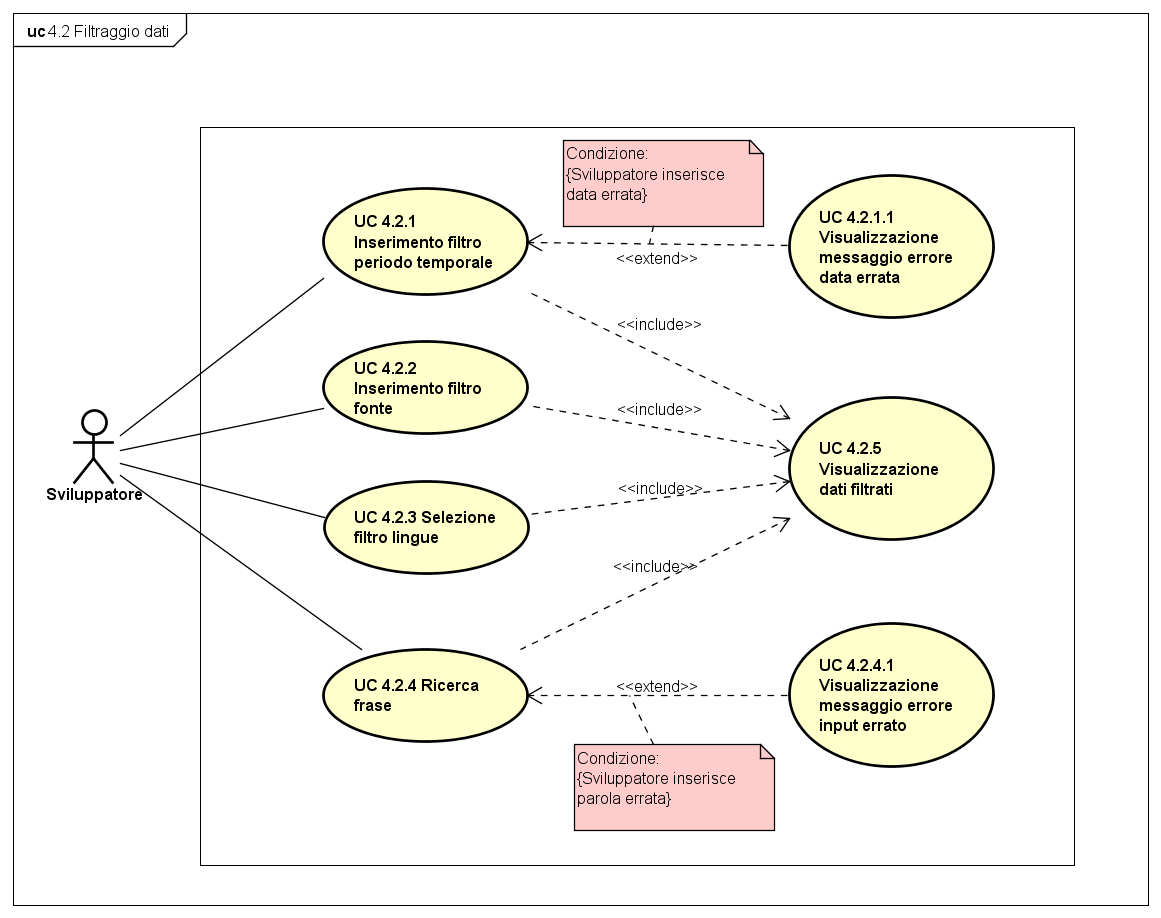
\includegraphics[width=17cm]{img/UC420.png} 
\caption{Caso d'uso 4.2}\label{fig:420}
\end{figure}
\begin{itemize}
\item[•]\textbf{Attori}: Sviluppatore;
\item[•]\textbf{Descrizione}: Lo sviluppatore applica dei filtri ai dati, ottenendo solo quelli d'interesse;
\item[•]\textbf{Precondizione}: Lo sviluppatore visualizza le proposizioni in ordine cronologico;
\item[•]\textbf{Postcondizione}: Lo sviluppatore visualizza i dati che rispettano i filtri scelti;
\item[•]\textbf{Flusso degli eventi principale}:
\begin{enumerate}
\item UC 4.2.1 Inserimento filtro periodo temporale;
\item UC 4.2.2 Inserimento filtro fonte\ped{G};
\item UC 4.2.3 Visualizzazione storico frase;
\item UC 4.2.4 Selezione filtro lingue;
\item UC 4.2.5 Ricerca parole chiave.
\end{enumerate}
\item[•]\textbf{Inclusioni}:
\begin{enumerate}
\item UC 4.2.6 - Visualizzazione dati filtrati
\end{enumerate}
\end{itemize}
\subsubsection{UC 4.2.1 - Inserimento filtro periodo temporale}
\begin{itemize}
\item[•]\textbf{Attori}: Sviluppatore;
\item[•]\textbf{Descrizione}: Lo sviluppatore seleziona un periodo temporale, ottenendo i dati salvati in un determinato arco di tempo;
\item[•]\textbf{Precondizione}: Lo sviluppatore visualizza le proposizioni in base ai filtri stabiliti;
\item[•]\textbf{Postcondizione}: Lo sviluppatore visualizza le frasi in base al filtraggio inserito;
\item[•]\textbf{Flusso degli eventi principale}: 
\begin{enumerate}
\item Scelta data inizio periodo
\item Scelta data fine periodo
\end{enumerate}
\item[•]\textbf{Estensioni}: 
\begin{enumerate}
	\item Visualizzazione messaggio di errore nel caso si scegliesse una data non idonea;
\end{enumerate}
\item[•]\textbf{Inclusioni}:
\begin{enumerate}
\item UC 4.2.6 - Visualizzazione dati filtrati
\end{enumerate}
\end{itemize}

\subsubsection{UC 4.2.2 - Inserimento filtro fonte}
\begin{itemize}
\item[•]\textbf{Attori}: Sviluppatore;
\item[•]\textbf{Descrizione}: Lo sviluppatore seleziona una o più fonti degli esercizi, come ad esempio le correzione provenienti da determinati docenti o dal sistema di correzione automatico;
\item[•]\textbf{Precondizione}: Lo sviluppatore visualizza le proposizioni in base ai filtri stabiliti;
\item[•]\textbf{Postcondizione}: Lo sviluppatore ha impostato i valori del filtro fonte;
\item[•]\textbf{Flusso degli eventi principale}: Lo sviluppatore seleziona da un elenco le fonti di cui è interessato visualizzare i dati;
\item[•]\textbf{Inclusioni}:
\begin{enumerate}
\item UC 4.2.6 - Visualizzazione dati filtrati
\end{enumerate}
\end{itemize}

\subsubsection{UC 4.2.3 -  Selezione filtro lingue}
\begin{itemize}
\item[•]\textbf{Attori}: Sviluppatore;
\item[•]\textbf{Descrizione}: Lo sviluppatore seleziona una o più lingue da un elenco di lingue predefinito al fine di ottenere solamente le proposizioni scritte in tali lingue;
\item[•]\textbf{Precondizione}: Lo sviluppatore visualizza le proposizioni in base ai filtri stabiliti;
\item[•]\textbf{Postcondizione}: Lo sviluppatore ha stabilito i valori di filtraggio relativi alle lingue;
\item[•]\textbf{Flusso degli eventi principale}: Lo sviluppatore seleziona da un elenco le lingue di cui è interessato vedere le proposizioni memorizzate;
\item[•]\textbf{Inclusioni}:
\begin{enumerate}
\item UC 4.2.6 - Visualizzazione dati filtrati
\end{enumerate}
\end{itemize}

\subsubsection{UC 4.2.4 - Ricerca frase}
\begin{itemize}
\item[•]\textbf{Attori}: Sviluppatore;
\item[•]\textbf{Descrizione}: Lo sviluppatore scrive una o più parole chiave al fine di cernere le frasi contenenti tali parole;
\item[•]\textbf{Precondizione}: Lo sviluppatore visualizza le frasi in base al filtraggio scelto;
\item[•]\textbf{Postcondizione}: Lo sviluppatore ha impostato le parole chiave;
\item[•]\textbf{Flusso degli eventi principale}: Lo sviluppatore seleziona da un elenco le lingue di cui è interessato vedere le proposizioni memorizzate;
\item[•]\textbf{Estensioni}: 
\begin{enumerate}
	\item Visualizzazione messaggio di errore nel caso venga inserito un input non consentito;
\end{enumerate}
\item[•]\textbf{Inclusioni}:
\begin{enumerate}
\item UC 4.2.6 - Visualizzazione dati filtrati
\end{enumerate}
\end{itemize}

\subsubsection{UC 4.2.6 - Visualizzazione dati filtrati}
\begin{itemize}
\item[•]\textbf{Attori}: Sviluppatore;
\item[•]\textbf{Descrizione}: Selezionato uno o più filtri, i dati vengono mostrati secondo i vincoli inseriti;
\item[•]\textbf{Precondizione}: I valori di uno o più filtri sono stati inseriti;
\item[•]\textbf{Postcondizione}: I dati mostrati rispettano tali vincoli;
\end{itemize}
